\section{The Rodin Platform}
\label{rodin_platform}
\index{Rodin}

In this section, we describe the details of the tool platform, as it is presented to the user.  You will find a description of all GUI elements that you may encounter.

\subsection{Eclipse in General}
\label{eclipse}
\index{Eclipse}

\textbf{From the Eclipse Website\footnote{\url{http://www.eclipse.org/}}:}
Eclipse is an open source community, whose projects are focused on building an open development platform comprised of extensible frameworks, tools and runtimes for building, deploying and managing software across the lifecycle. The Eclipse Foundation is a not-for-profit, member supported corporation that hosts the Eclipse projects and helps cultivate both an open source community and an ecosystem of complementary products and services.

\textbf{From Wikipedia\footnote{\url{http://en.wikipedia.org/}}:}
Eclipse is a multi-language software development environment comprising an integrated development environment (IDE) and an extensible plugin system. It is written mostly in Java and can be used to develop applications in Java and, by means of various plugins, other programming languages including Ada, C, C++, COBOL, Perl, PHP, Python, R, Ruby (including Ruby on Rails framework), Scala, Clojure, Groovy and Scheme. It can also be used to develop packages for the software Mathematica. The IDE is often called Eclipse ADT (Ada Development Toolkit) for Ada, Eclipse CDT for C/C++, Eclipse JDT for Java, and Eclipse PDT for PHP.

Eclipse provides the technical foundation of Rodin.

\subsubsection{Project Constituents and Relationships}
\label{project}
\index{project}

The primary concept in doing formal developments with the Rodin Platform is that of a project. A project contains the complete mathematical development of a Discrete Transition System. It is made of several components of two kinds: machines and contexts. Machines contain the variables, invariants, theorems, and events of a project, whereas contexts contain the carrier sets, constants, axioms, and theorems of a project. Figure \ref{fig_ref_10_project1} shows an overview.

\begin{figure}[!ht]
\begin{center}
	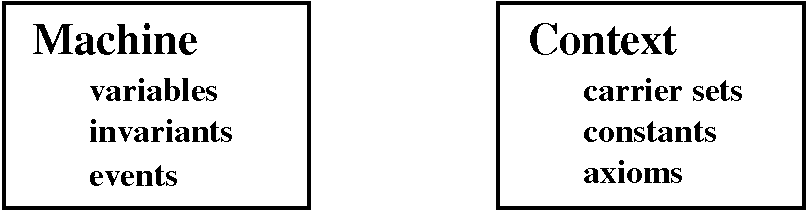
\includegraphics{img/reference/ref_10_project1.png}
	\caption{Overview Machine and Context}
	\label{fig_ref_10_project1}
\end{center}
\end{figure}

We remind the reader of the various relationships existing between machines and contexts. This is illustrated in the following figure. A machine can be ``refined" by another one, and a context can be ``extended" by another one (no cycles are allowed in both these relationships). Moreover, a machine can ``see" one or several contexts. A typical example of machine and context relationship is shown in Figure \ref{fig_ref_10_project2}. 

\begin{figure}[!ht]
\begin{center}
	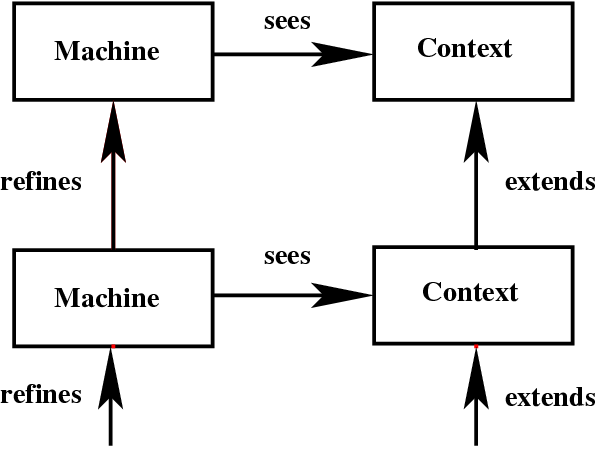
\includegraphics{img/reference/ref_10_project2.png}
	\caption{A typical example of machine and context relationship}
	\label{fig_ref_10_project2}
\end{center}
\end{figure}

\subsubsection{Rodin Nature}
\label{rodin_nature}

Eclipse Projects can have one or more natures to describe their purpose.  The GUI can then adapt to their nature.  Rodin Projects must have the Rodin-Nature.  If you create an Event-B project, it automatically has the right nature.  If you want to modify an existing project, you can edit the \texttt{.project} file and add the following XML in the \texttt{<natures>} section:

\pencil{
\texttt{<nature>org.rodinp.core.rodinnature</nature>}
}


\subsection{The Event-B Perspective}
\label{event_b_perspective}
\index{Event-B!perspective}
\index{perspective!Event-B}

\marginpar{Screenshots must be adapted to Rodinv2.4}

Figure \ref{fig_ref_01_eventb_perspective1} shows an overview of the opening window of the Event-B Perspective. The following subsections identify the different Rodin GUI elements (i.e. Views) which are visible and explain their functions.

\imagedpi{img/reference/ref_01_eventb_perspective1.pdf}{150mm}{img/reference/ref_01_eventb_perspective1.png}{Overview of the Event-B Perspective}{fig_ref_01_eventb_perspective1}

\subsubsection{Menu bar}
\label{menu_bar}

The menu bar provides file and edit operations and other useful Event-B specific operations. We will briefly describe the most important menu items here.

\paragraph{Rename menu}

When opening a machine or context file, the following actions for automatically renaming the Event-B model elements are available for the user:

One action is available when editing context files (see Figure \ref{fig_ref_01_menubar1}).

    \begin{itemize}
    	\item Automatic Axiom Labelling: this action will rename the axioms alphanumerically renaming according to their order of appearance. 
    \end{itemize}

\begin{figure}[!ht]
\begin{center}
	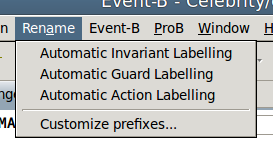
\includegraphics{img/reference/ref_01_menubar1.png}
	\caption{Automatic rename actions for machine files}
	\label{fig_ref_01_menubar1}
\end{center}
\end{figure}

Three actions are available for machine files (see Figure \ref{fig_ref_01_menubar2}).

    \begin{itemize}
    	\item Automatic Invariant Labelling: this action will rename the invariants alphanumerically according to their order of appearance.
	\item Automatic Guard Labelling: this action will rename the guards alphanumerically according to their order of appearance,
	\item Automatic Action Labelling: this action will rename the actions alphanumerically according to their order of appearance. 
    \end{itemize}

\begin{figure}[!ht]
\begin{center}
	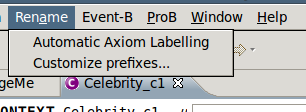
\includegraphics{img/reference/ref_01_menubar2.png}
	\caption{Automatic rename actions for context files}
	\label{fig_ref_01_menubar2}
\end{center}
\end{figure}

\paragraph{Event-B menu}

When opening a machine or context file, some wizards for creating Event-B model elements are available for the user. The different wizards are described in Section \ref{eventb_editor}.

\subsubsection{Tool bar}
\label{tool_bar}

The tool bar provides short cuts for familiar commands like save, print, undo and redo. The tool bar also provides short cuts to the wizards for creating elements like axioms, constants, enumerated sets, etc., which are described in Section \ref{eventb_editor}.

\subsubsection{Editor View}
\label{editor_view}

The editor view contains the active Event-B editor which is described in Section \ref{eventb_editor}.

\subsubsection{Outline View}
\label{outline_view}

The outline view displays the outline of the active Event-B editor and lists elements like axioms, variables, etc.. 

\subsubsection{Rodin Problems View}
\label{rodin_problems_view}
\index{Rodin problems view}
\index{view!Rodin Problems view}

When the Static Checker discovers an error in a project, a \icon{rodin/error_ovr.png} marker is added to this project and to the faulty component in the \textsf{Event-B Explorer}. The error itself is shown in the Rodin Problems view (i.e. syntax errors) of the active Event-B editor.

By double-clicking on the error statement, you are transferred automatically into the place where the error has been detected so that you can correct it easily.

\subsubsection{Symbols View}
\label{symbols_view}
\index{view!Symbols View}

The symbols view is intended to give users a convenient way to type in mathematical symbols into the various model editors. If an editor is open and a text field is active (the cursor is blinking), then clicking a symbol inserts it at the current position as demonstrated in Figure \ref{fig_ref_01_symbol_table1}. 

The ASCII code corresponding to the symbol over which the mouse hovers is also displayed as a tooltip so that the user can also learn how to input symbols directly. 

\begin{figure}[!ht]
\begin{center}
	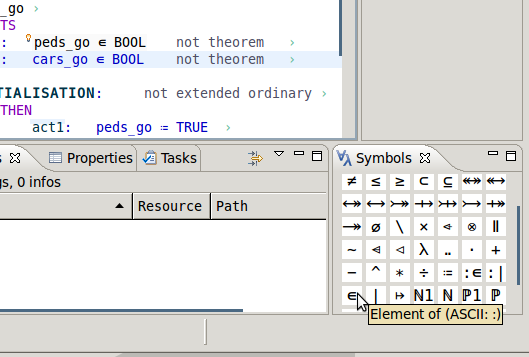
\includegraphics{img/reference/ref_01_symbol_table1.png}
	\caption{Clicking a symbol inserts it at the current position}
	\label{fig_ref_01_symbol_table1}
\end{center}
\end{figure}

\subsubsection{Event-B Explorer}
\label{eventb_explorer}
\index{Event-B!explorer}

Projects can be found in the RODIN platform in the \textsf{Event-B Explorer}. This is usually situated on the left hand side of the screen as shown in Figure \ref{fig_ref_01_eventb_perspective1}. The \textsf{Event-B Explorer} contains a list of name of the current projects. Next to each project name is a small triangle. By pressing it, one can expand a project and see the machines and contexts that it contains.

The icons (\icon{rodin/ctx_obj.png} or \icon{rodin/mch_obj.png}) next to the components help identify whether they are a context or machine respectively.

When expanding a machine or a context, you can explore its elements. Double clicking on a specific element (i.e. a variable) opens the Event-B editor and marks the position of the variable in the machine or context as shown in Figure \ref{fig_ref_01_project_explorer1}. Furthermore, proof obligations are displayed when clicking on the small triangle next to the label \textsf{Proof Obligations} (for more information see Section \ref{proving_perspective}).

\begin{figure}[!ht]
\begin{center}
	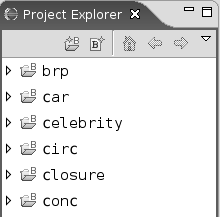
\includegraphics{img/reference/ref_01_project_explorer1.png}
	\caption{Double clicking on an element opens the Event-B editor and marks the corresponding position}
	\label{fig_ref_01_project_explorer1}
\end{center}
\end{figure}

\subsection{Customizing a perspective suitable for RODIN}
\label{customizing_a_perspective_suitable_for_rodin}
\index{perspective!customization}
\index{fast view bar}

So far, you have needed two different perspectives to work with RODIN. But it actually is possible to work with only one perspective. In this section, we try to customize a perspective so that we do not need any other. If you have experience with customizing Eclipse perspectives, you may only want to read the next paragraph which contains a few thoughts about a good perspective for RODIN.

As a start, we should think about what we want the perspective to look like. The proving perspective already is quite nice, but we may want to use a little bit more editing space when in the Event-B perspective. To create more space, we could move all windows that currently are on both sides of the editing area onto one side, as they never really need to be used simultaneously. For a bit more space, we could dock all of these windows onto the so-called Fast View bar so that they disappear when they are not needed. It would also be nice to be able to split the screen and work on several compontents at once. For example, we could have an abstract machine on one side of the editing surface, and the concrete machine on the other.

For the most part, the perspectives can be customized by dragging and dropping the different windows. First of all, you need to find the Fast View Bar. Usually, it is at the bottom end of the Eclipse window, but it also can be on the side or hidden inside the Shortcut Bar. For our purposes, it probably is best to have it on the right side of the screen. Place it there by dragging it with the mouse. Now, add some items to it. To do this, press the \textsf{New Fast View} button on the bar. It might be better to leave the Goal, the Problems and the Proof Control window at the bottom of the screen, as you may want them to stay open while editing. A good selection of tools to add to the Fast View bar may be:

\begin{itemize}
	\item Project Explorer
	\item Obligation Explorer
	\item Search Hypothesis
	\item Cache Hypothesis
	\item Proof Tree
	\item Proof Information
	\item Progress Window
\end{itemize}

All of the windows that you cannot create directly when clicking on \textsf{New Fast View} can be found under \textsf{Others/General}. Once you are done, the window should look like in Figure \ref{fig_ref_10_customizing}. Click on ``Save Perspective As…'' in the Window menu to save the perspective.

\begin{figure}[!ht]
\begin{center}
	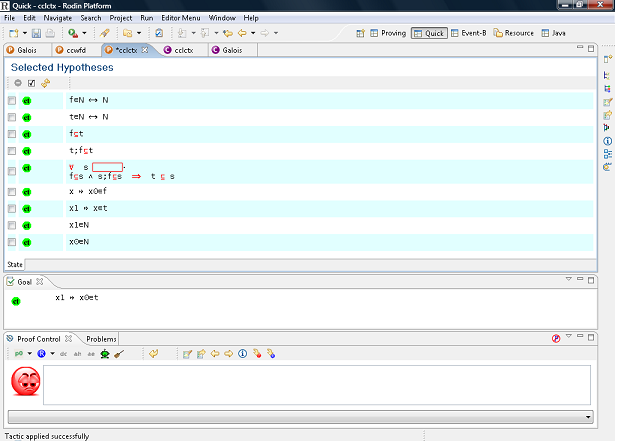
\includegraphics{img/reference/ref_10_customizing.png}
	\caption{Our self-made Quick perspective}
	\label{fig_ref_10_customizing}
\end{center}
\end{figure}

\subsection{The Event-B Editor}
\label{new_eventb_editor}
\index{editor!default editor}

Once a context or a machine is created, a window appears in the editing area as shown in figure \ref{fig_ref_01_eventb_editor1_neweditor}.

\warning{The editor described here was made the default editor in Rodin 2.4 (February 2012) and still has some minor issues (see section~\ref{faq_new_editor_new_element}, for instance).  The alternative structural editor is still available, see section~\ref{eventb_editor}.}

\begin{figure}[!ht]
\begin{center}
	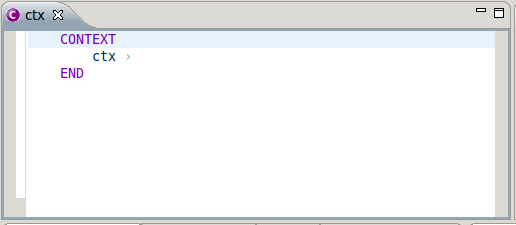
\includegraphics{img/reference/ref_01_eventb_editor1_neweditor.png}
	\caption{The Event-B editor}
	\label{fig_ref_01_eventb_editor1_neweditor}
\end{center}
\end{figure}

The editor allows you to edit the modelling elements of the context which are the dependencies, the carrier sets, the constants, and the axioms. By right-clicking on predefined places you can create new modelling elements. For instance, there is a small green arrow directly to the right of the name of the context (in this case, the name of the context is "ctx"). Place your cursor directly to the left of the green arrow and right click. Select the element that you would like to add from the \textsf{Add Child} menu as shown in figure \ref{fig_ref_01_neweditor_add_element}.

\begin{figure}[!ht]
\begin{center}
	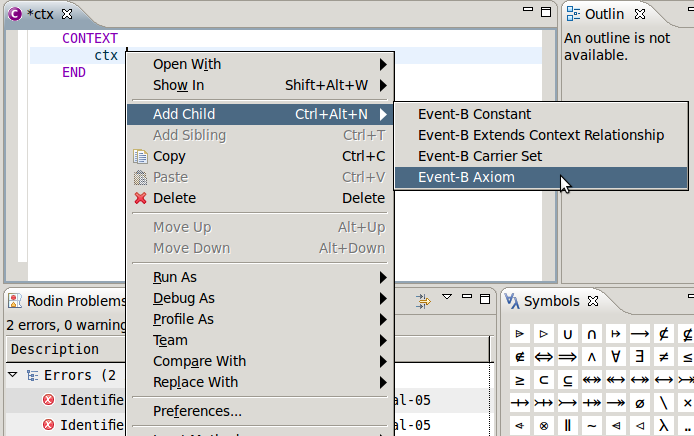
\includegraphics{img/reference/ref_01_neweditor_add_element.png}
	\caption{Adding a new modelling element}
	\label{fig_ref_01_neweditor_add_element}
\end{center}
\end{figure}

To remove a modelling element, right click on the modelling element and select \textsf{Delete}.

It is also possible to add modelling elements by using wizards (See \ref{eventb_editor}).

\subsection{The Structural Event-B Editor}
\label{eventb_editor}
\index{editor!structural editor}

\info{The editor described here was the default editor until Rodin 2.3.  It is still available, but has to be stared explicitly through the context menu of the Component.}

Once a context or a machine is created, a window appears in the editing area as shown in figure \ref{fig_ref_01_eventb_editor1}.

\begin{figure}[!ht]
\begin{center}
	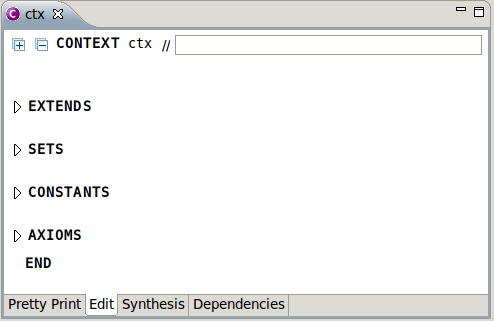
\includegraphics{img/reference/ref_01_eventb_editor1.png}
	\caption{The Structured Event-B editor}
	\label{fig_ref_01_eventb_editor1}
\end{center}
\end{figure}

By default, you are in the \textsf{Edit} mode which allows you to edit the modelling elements of the context which are the dependencies, the carrier sets, the constants, and the axioms. By right-clicking on the modelling elements you can create new child and sibling elements. For instance,
By pressing the triangle (\icon{rodin/collapsed.png}) next to each keyword, you can see the different modelling elements and also add, remove, or move them. Figure \ref{fig_ref_01_eventb_editor2} shows what the section looks like after pressing the triangle next to the keyword "AXIOMS".

\begin{figure}[!ht]
\begin{center}
	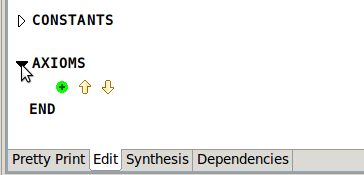
\includegraphics{img/reference/ref_01_eventb_editor2.png}
	\caption{By pressing the triangle you can collapse/expand context sections}
	\label{fig_ref_01_eventb_editor2}
\end{center}
\end{figure}

By pressing the \icon{rodin/add.png} button, you can add a new modelling element. For instance, clicking on the \icon{rodin/add.png} button next in the \textsf{AXIOMS} section will add a new axiom element. You can now enter a new axiom and a comment in the corresponding boxes as indicated in Figure \ref{fig_ref_01_eventb_editor3}.

\begin{figure}[!ht]
\begin{center}
	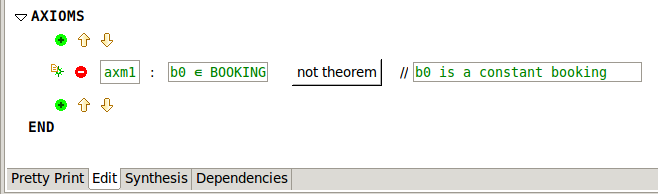
\includegraphics{img/reference/ref_01_eventb_editor3.png}
	\caption{Adding a new modelling element}
	\label{fig_ref_01_eventb_editor3}
\end{center}
\end{figure}

To remove a modelling element, press the \icon{rodin/remove.png} button. You can also move an modelling element up or down by selecting it and then pressing one of the two arrows (\icon{rodin/up_edit.png} or \icon{rodin/down_edit.png}).

It is also possible to add modelling elements by using wizards. You can active the different wizard by using the buttons in the tool bar as shown in Figure \ref{fig_ref_01_eventb_editor12} and in Figure \ref{fig_ref_01_eventb_editor13} or via the Event-B menu (keeping in mind that the wizards depend on the active file machine or context). The next sections explain how to use the wizards.

\begin{figure}[!ht]
\begin{center}
	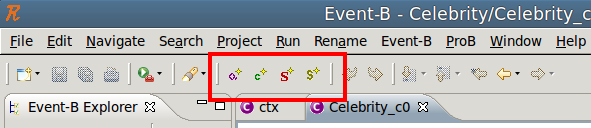
\includegraphics{img/reference/ref_01_eventb_editor12.png}
	\caption{Wizards for context specific elements located in the tool bar}
	\label{fig_ref_01_eventb_editor12}
\end{center}
\end{figure}

\begin{figure}[!ht]
\begin{center}
	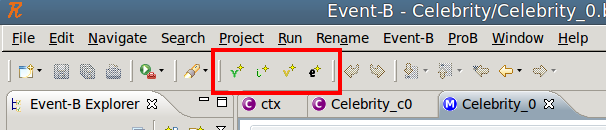
\includegraphics{img/reference/ref_01_eventb_editor13.png}
	\caption{Wizards for machine specific elements located in the tool bar}
	\label{fig_ref_01_eventb_editor13}
\end{center}
\end{figure}


\subsubsection{New Carrier Sets Wizard}
\index{wizard!New Carrier Sets Wizard}

To activate the \textsf{New Carrier Sets Wizard}, press the \icon{rodin/newset_edit.png} button located in the tool bar. Pressing the button bring up the window shown in Figure \ref{fig_ref_01_eventb_editor4}.

\begin{figure}[!ht]
\begin{center}
	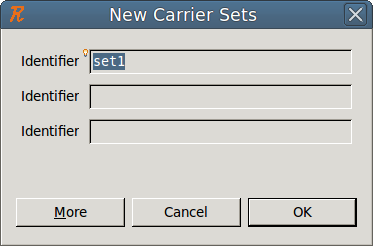
\includegraphics{img/reference/ref_01_eventb_editor4.png}
	\caption{New Carrier Sets Wizard}
	\label{fig_ref_01_eventb_editor4}
\end{center}
\end{figure}

You can enter as many carrier sets as you want by pressing the \textsf{More} button. When you are finished, press the \textsf{OK} button. 

\subsubsection{New Enumerated Set Wizard}
\label{enumerated_set_wizard}
\index{wizard!New Enumerated Set Wizard}

To activate the \textsf{New Enumerated Set Wizard}, press the \icon{rodin/newenuset_edit.png} button located in the tool bar. Pressing the button bring up the window shown in Figure \ref{fig_ref_01_eventb_editor5}.

\begin{figure}[!ht]
\begin{center}
	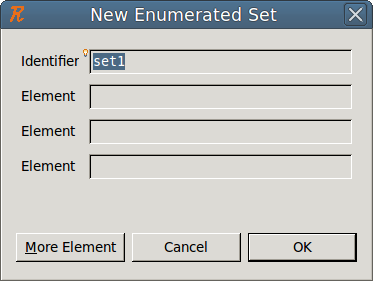
\includegraphics{img/reference/ref_01_eventb_editor5.png}
	\caption{New Enumerated Set Wizard}
	\label{fig_ref_01_eventb_editor5}
\end{center}
\end{figure}

Enter the name of the new enumerated set as well as the names of its elements. By pressing the \textsf{More Elements} button, you can enter additional elements. When you're finished, press the \textsf{OK} button. The benefit of using this wizard is that in addition to creating the set and its elements, the wizard automatically creates the axiom that is necessary for the context to work. For example, when you add the new carrier set \texttt{COLOUR} and the three constants \texttt{red}, \texttt{green}, and \texttt{orange}, the wizard automatically creates the following axiom $partition(COLOUR , \{red\}, \{green\}, \{orange\})$.

\subsubsection{New Constants Wizard}
\index{wizard!New Constants Wizard}

To activate the \textsf{New Constants Wizard}, press the \icon{rodin/newcst_edit.png} button located in the tool bar. Pressing the button will bring up the window shown in Figure \ref{fig_ref_01_eventb_editor6}.

\begin{figure}[!ht]
\begin{center}
	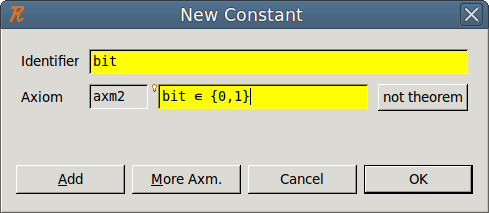
\includegraphics{img/reference/ref_01_eventb_editor6.png}
	\caption{New Constants Wizard}
	\label{fig_ref_01_eventb_editor6}
\end{center}
\end{figure}

You can then enter the names of a constant and an axiom which can be used to define the constant's type. By pressing the \textsf{More Axm.} button you can enter additional axioms. To add more constants, press the \textsf{Add} button. When you have finished, press the \textsf{OK} button.

\subsubsection{New Axioms Wizard}
\index{wizard!New Axioms Wizard}

To activate the \textsf{New Axioms Wizard}, press the \icon{rodin/newaxm_edit.png} button located in the tool bar. Pressing the button brings up the window shown in Figure \ref{fig_ref_01_eventb_editor7}.

\begin{figure}[!ht]
\begin{center}
	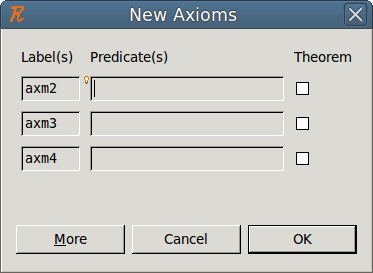
\includegraphics{img/reference/ref_01_eventb_editor7.png}
	\caption{New Axioms Wizard}
	\label{fig_ref_01_eventb_editor7}
\end{center}
\end{figure}

You can then enter the axioms you want. If more axioms are needed, press the \textsf{More} button. When you are finished, press the \textsf{OK} button.

Check the ``Theorem" checkbox to indicate that the corresponding axiom should be a theorem.

\subsubsection{New Variable Wizard}
\index{wizard!New Variable Wizard}

To activate the \textsf{New Variable Wizard}, press the \icon{rodin/newvar_edit.png} button located in the tool bar. Pressing the button brings up the window shown in Figure \ref{fig_ref_01_eventb_editor14}.

\begin{figure}[!ht]
\begin{center}
	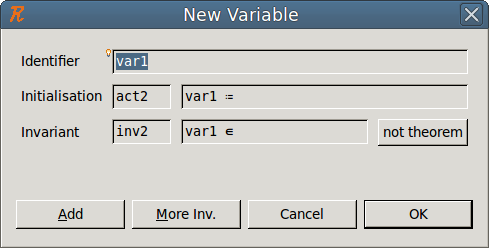
\includegraphics{img/reference/ref_01_eventb_editor14.png}
	\caption{New Variable Wizard}
	\label{fig_ref_01_eventb_editor14}
\end{center}
\end{figure}

You can then enter the names of the variable, what its state at initialization should be, and an invariant which defines its type. By pressing button \textsf{More Inv.}, you can enter additional invariants. For adding more variables, press the \textsf{Add} button. When you're finished, press the \textsf{OK} button. 

\subsubsection{New Invariants Wizard}
\index{wizard!New Invariants Wizard}

To activate the \textsf{New Invariants Wizard}, press the \icon{rodin/newinv_edit.png} button located in the tool bar. Pressing the button bring up the window shown in Figure \ref{fig_ref_01_eventb_editor15}.

\begin{figure}[!ht]
\begin{center}
	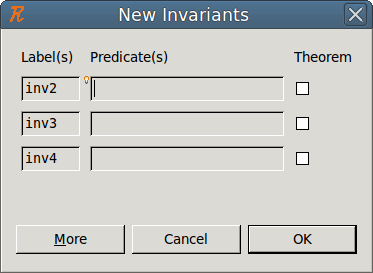
\includegraphics{img/reference/ref_01_eventb_editor15.png}
	\caption{New Invariants Wizard}
	\label{fig_ref_01_eventb_editor15}
\end{center}
\end{figure}

You can then enter the invariants you want. If more invariants are needed, press the \textsf{More} button. Check the \textsf{Theorem} checkbox to indicate that the corresponding invariant should be a theorem.

\subsubsection{New Event Wizard}
\index{wizard!New Event Wizard}

To activate the \textsf{New Events Wizard}, press the \icon{rodin/newevt_edit.png} button located in the tool bar. Pressing this button brings up the window shown in Figure \ref{fig_ref_01_eventb_editor16}.

\begin{figure}[!ht]
\begin{center}
	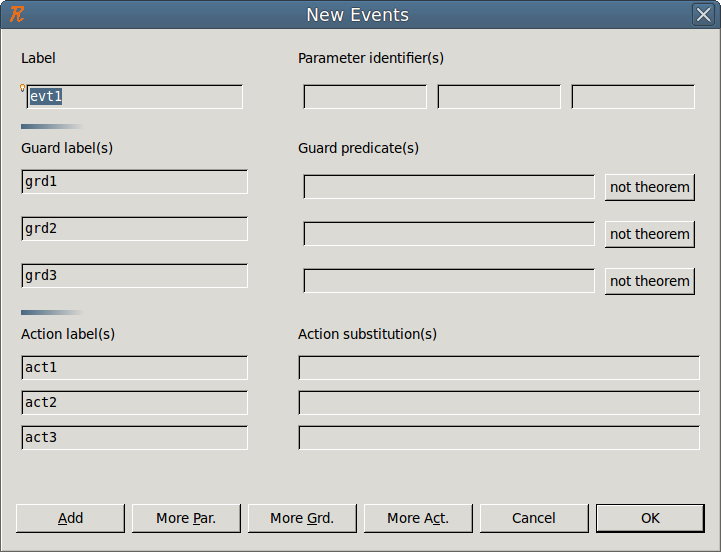
\includegraphics{img/reference/ref_01_eventb_editor16.png}
	\caption{New Event Wizard}
	\label{fig_ref_01_eventb_editor16}
\end{center}
\end{figure}

You can then enter the events that you want. As indicated, the following elements can be entered: name, parameters, guards, and actions. More parameters, guards and actions can be entered by pressing the corresponding buttons. If more events are needed, press the \textsf{Add} button. Press the \textsf{OK} button when you're finished.

Note that an event with no guard is considered to the guard $true$. Also, an event with no action is considered to have the action $skip$. 

\subsubsection{Dependencies (Context)}
\index{context!dependencies}

By selecting the \textsf{Dependencies} tab at the bottom of the Event-B editor, you obtain the window as shown in Figure \ref{fig_ref_01_eventb_editor8}.

\begin{figure}[!ht]
\begin{center}
	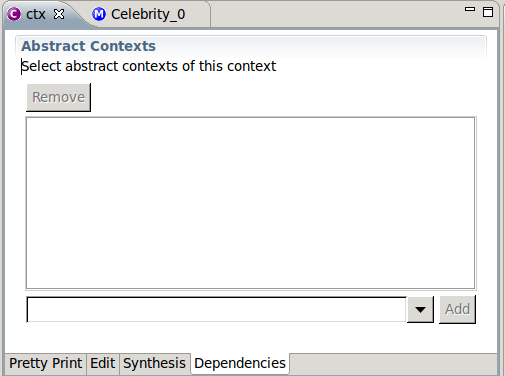
\includegraphics{img/reference/ref_01_eventb_editor8.png}
	\caption{Dependencies tab of the Event-B editor}
	\label{fig_ref_01_eventb_editor8}
\end{center}
\end{figure}

The dependencies tab allows you to control what other contexts that the current context is extending. To add the context that you want to extend, select the name of the context from the drop-down menu at the bottom of the window and then hit the \textsf{Add} button.

There is also another way to create a new context as an extension existing one. Select the context in the project window and then press the right mouse key. Then select \textsf{Extend} from the menu that opens up. This should bring up the window as shown in Figure \ref{fig_ref_01_eventb_editor9}.

\begin{figure}[!ht]
\begin{center}
	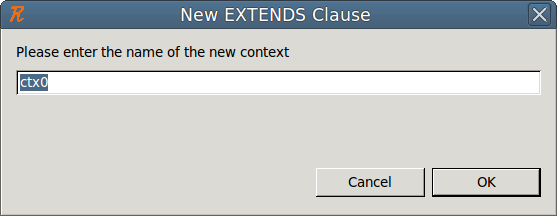
\includegraphics{img/reference/ref_01_eventb_editor9.png}
	\caption{New EXTENDS Clause window}
	\label{fig_ref_01_eventb_editor9}
\end{center}
\end{figure}

You can then enter the name of the new context which will automatically extend your chosen context. 

\subsubsection{Dependencies (Machine)}
\index{machine!dependencies}

The \textsf{Dependencies} tab for machines is very similar to the one for contexts that is described in the previous section. The main difference is that there are two kinds of dependencies that can be established: machines on which the current machine depends are listed in the upper part and contexts on which the current machine depends are listed in the lower part.

\subsubsection{Synthesis (Context)}
\index{context!synthesis}

Selecting the \textsf{Synthesis} tab brings up a global view of your context's elements (carrier set / constant / axiom / extended context) as demonstrated in Figure \ref{fig_ref_01_eventb_editor11}. 

\begin{figure}[!ht]
\begin{center}
	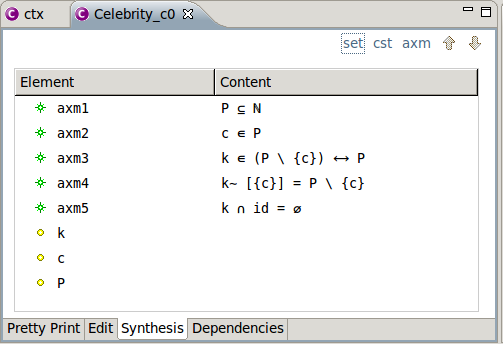
\includegraphics{img/reference/ref_01_eventb_editor11.png}
	\caption{The Synthesis tab of the Event-B editor}
	\label{fig_ref_01_eventb_editor11}
\end{center}
\end{figure}

By pressing the \textsf{set}, \textsf{cst}, or \textsf{axm} buttons in the upper right corner, you can filter out the carrier sets, constants or axioms of your context respectively.

If you select an element, you can change its priority by pressing the \icon{rodin/up_edit.png} button or the \icon{rodin/down_edit.png} button‎. You do this for axioms, carrier sets, constants and extended contexts.

Right clicking in this view will bring up a contextual menu that allows you to add a new carrier set, constant, axiom or extended context. 

\subsubsection{Synthesis (Machine)}
\index{machine!synthesis}

The \textsf{Synthesis} tab for machines is very similar to the one of contexts (see above) except that you have a global view of your machine's elements (refined machine/seen context/variable/invariant/event/variant).

\subsubsection{Pretty Print}
\index{pretty print}

Selecting the \textsf{Pretty Print} tab gives you a global view of your context or machine as if it had been entered through with an input text file as seen in Figure \ref{fig_ref_01_eventb_editor10}.

\begin{figure}[!ht]
\begin{center}
	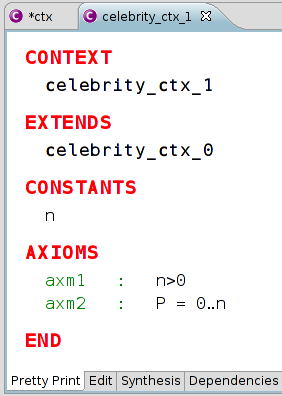
\includegraphics{img/reference/ref_01_eventb_editor10.png}
	\caption{The Pretty Print tab of the Event-B editor}
	\label{fig_ref_01_eventb_editor10}
\end{center}
\end{figure}

\subsection{The Proving Perspective}
\label{proving_perspective}
\index{perspective!proving}
\index{proving!perspective}

When proof obligations (POs) (Section \ref{generated_proof_obligations}) are not discharged automatically, the user can attempt to discharge them interactively using the Proving Perspective. This page provides an overview of the Proving Perspective and its use. If the Proving Perspective is not visible as a tab on the top right-hand corner of the main interface, the user can switch to it via \textsf{Window $\rangle$ Open Perspective}.

The Proving Perspective consists of a number of views: the \textsf{Proof Tree}, the \textsf{Goal}, the \textsf{Selected Hypotheses}, the \textsf{Proof Control}, the \textsf{Search Hypotheses}, the \textsf{Cache Hypotheses} and the \textsf{Proof Information}. In the discussion that follows we look at each of these views individually. Figure \ref{fig_ref_01_proving_perspective1} shows an overview of the Proving Perspective.

\imagedpi{img/reference/ref_01_proving_perspective1.pdf}{150mm}{img/reference/ref_01_proving_perspective1.png}{Overview of the Proving Perspective}{fig_ref_01_proving_perspective1}

\subsubsection{Loading a Proof}

To work on an PO that has not yet been discharged, it is necessary to load the proof into the Proving Perspective. To do this, switch to the Proving Perspective. Select the project from the Event-B Explorer and select and expand the component (context or machine). Finally, select (double-click) the proof obligation of interest. A number of views will be updated with details of the corresponding proof. 

Note that pressing the \icon{rodin/discharged.png} button on the top left hand side of the \textsf{Event-B Explorer} will remove all discharged proof obligations (PO's) from the view. 

\subsubsection{The Proof Tree}
\label{proof_tree_view}
\index{proving!the proof tree}

The proof tree view provides a graphical representation of each individual proof step as seen in figure \ref{fig_ref_01_proving_perspective2}.

\begin{figure}[!ht]
\begin{center}
	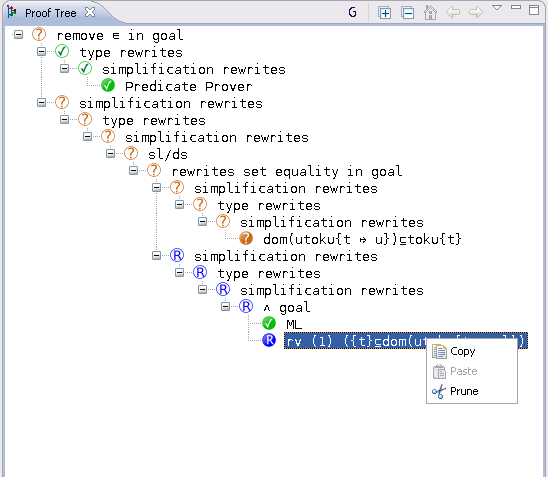
\includegraphics{img/reference/ref_01_proving_perspective2.png}
	\caption{The Proof Tree}
	\label{fig_ref_01_proving_perspective2}
\end{center}
\end{figure}

The tree is made up of sequents. A line of the tree is shifted to the right when the corresponding node is a direct descendant of the node of the previous line. Each sequent is labeled with a comment which indicates which rule has been applied or which prover discharged the proof. By selecting a sequent in the proof tree, the hypotheses of the sequent are loaded to the \textsf{Selected Hypotheses window}, and the goal of the sequent is loaded to the \textsf{Goal view}.

\paragraph{Decoration}
\index{reviewed}
\index{pending}
\index{discharged}
The symbol to the left of the leaf indicates the state of the sequent:
\begin{itemize}
	\item \icon{rodin/discharged.png} indicates that this sequent is discharged.
	\item \icon{rodin/pending.png} indicates that this sequent is not discharged.
	\item \icon{rodin/reviewed.png} indicates that this sequent has been reviewed. 
\end{itemize}

Internal nodes in the proof display the symbols in reverse colours. Note that a ``reviewed" sequent is one that is not discharged yet by the prover. Instead, it has been ``seen" by the user who decided to postpone the proof. Marking sequents as ``reviewed" is very convenient since the provers will ignore these leaves and focus on specific areas of interest. This allows the proof to be discharged interactively in a gradual fashion. In order to discharge a ``reviewed" sequent, select it and prune the tree at that node: the node will become ``brown" again (undischarged), and you can now try to discharge it. 

\paragraph{Navigation within the Proof Tree}

There are three buttons on the top of the proof tree view:

\begin{itemize}
	\item \icon{rodin/showgoal.png} allows you to see the goal of corresponding to each. node,
	\item \icon{rodin/collapseall.png} allows you to fully expand the proof tree.
	\item \icon{rodin/expandall.png} allows you to fully collapse the tree; only the root stays visible. 
\end{itemize}

\paragraph{Manipulating the Proof Tree}

\subparagraph{Hiding}

The button next to each node in the proof tree allows you to expand or collapse the subtree starting at that node. 

\subparagraph{Pruning}
\index{proving!pruning}

The proof tree can be pruned at a selected node. This means that the subtree of the selected node is removed from the proof tree. The selected node becomes a leaf and displays the symbol \icon{rodin/pending.png}. The proof activity can then be resumed from this node. After selecting a node in the proof tree, pruning can be performed in two ways:

\begin{itemize}
	\item by right-clicking and then selecting \textsf{Prune},
	\item by clicking on the \icon{rodin/pn_prover.png} button in the proof control view. 
\end{itemize}

Note that after pruning, the post-tactic is not applied to the new current sequent. The post-tactic should be applied manually, if required, by clicking on the post-tactic button in the Proof Control view. This is especially useful when you want to redo a proof from the beginning. The proof tree can be pruned at its root node and then the proof can proceed again with invocation of internal or external provers or with an interactive proof.

Before pruning a particular node, the node (and its subtree) can be copied to the clipboard. If the new proof strategy subsequently fails, the copied version can be pasted back into the pruned node (see the next section). 

\subparagraph{Copy/Paste}

By selecting a node in the proof tree and then right-clicking with the mouse, you can copy the part of the proof tree starting at that sequent (including the node and its subtree). Pasting the node and subtree back in is done in a similar manner with a right mouse click on a proof node. This allows reuse of part of a proof tree in the same or even in another proof.

\subsubsection{Goal and Selected Hypotheses}
\label{goal_view}
\index{goal}
\index{selected hypotheses}

Each sequent in the proof tree have corresponding hypotheses and goals. A user will work with one selected sequent at a time by attempting various strategies in an effort to show that the goal is true. The \textsf{Goal} and \textsf{Selected Hypotheses} views provide information to the user about the currently selected sequent. Figure \ref{fig_ref_01_proving_perspective3} shows an example.

\begin{figure}[!ht]
\begin{center}
	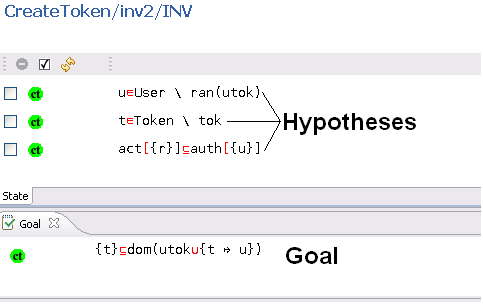
\includegraphics{img/reference/ref_01_proving_perspective3.png}
	\caption{Open proof obligation}
	\label{fig_ref_01_proving_perspective3}
\end{center}
\end{figure}

A hypothesis can be removed from the list of selected hypotheses by selecting the check the box situated next to it (you can click on several boxes at once) and then by clicking on the \icon{rodin/remove.png} button at the top of the selected hypotheses window.

Note that the deselected hypotheses are not lost. You can find them again using the \textsf{Search Hypotheses} \icon{rodin/sh_prover.png} button in the Proof Control view. Other buttons are used as follows:

\begin{itemize}
	\item \icon{rodin/select_all_prover.png} - Select all hypotheses. 
	\item \icon{rodin/inv_prover.png} - Invert the selection. 
	\item \icon{rodin/falsify_prover.png} next to the goal - Proof by contradiction 1: The negation of the goal becomes a selected hypothesis and the goal becomes ``$\bot$". 
	\item \icon{rodin/falsify_prover.png} next to a selected hypothesis - Proof by contradiction 2: The negation of the hypothesis becomes the goal and the negated goal becomes a selected hypothesis. 
\end{itemize}

A user wishing to attempt an interactive proof has a number of proof rules available, and these may either rewrite a hypothesis/goal or infer something from it. In the \textsf{Goal} and the \textsf{Selected Hypotheses} views, various operators may appear in red coloured font. The red font indicates that some interactive proof rule(s) are applicable and may be applied as a step in the proof attempt. When the mouse hovers over such an operator, a number of applicable rules may be displayed; the user may choose to apply one of the rules by clicking on it. Figure \ref{fig_ref_01_proving_perspective4} shows an example.

Other proof rules can be applied when green buttons appear in the \textsf{Goal} and \textsf{Selected Hypotheses} views. Examples are proof by contradiction \icon{rodin/falsify_prover.png} and conjunction introduction \icon{rodin/conjI_prover.png}. 

\begin{figure}[!ht]
\begin{center}
	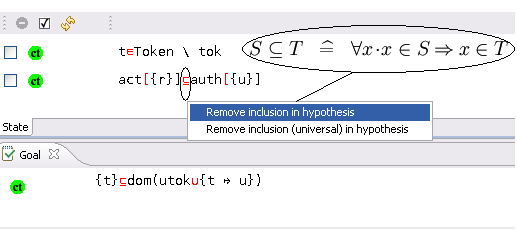
\includegraphics{img/reference/ref_01_proving_perspective4.png}
	\caption{Applying a rule}
	\label{fig_ref_01_proving_perspective4}
\end{center}
\end{figure}

To instantiate a quantifier, the user enters the desired expression in the box behind the quantifier and clicks on the quantifier (the red $\exists$) as demonstrated in figure \ref{fig_ref_01_proving_perspective5}.

\begin{figure}[!ht]
\begin{center}
	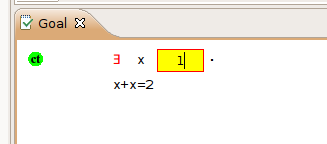
\includegraphics{img/reference/ref_01_proving_perspective5.png}
	\caption{Instantiating a quantifier}
	\label{fig_ref_01_proving_perspective5}
\end{center}
\end{figure}

\subsubsection{The Proof Control View}
\label{proof_control_view}
\index{proof control view}
\index{view!Proof Control}

The \textsf{Proof Control} view contains the buttons with which you can perform an interactive proof. An overview of this proof can be seen in Figure \ref{fig_ref_01_proving_perspective6}.

\begin{figure}[!ht]
\begin{center}
	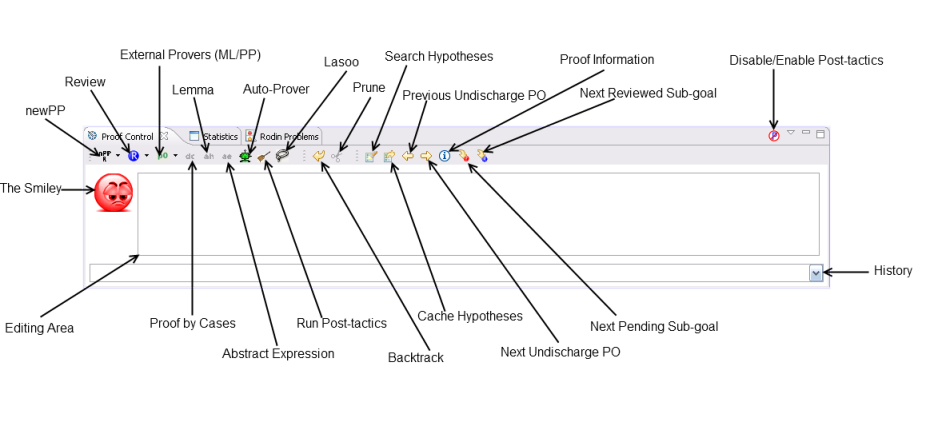
\includegraphics{img/reference/ref_01_proving_perspective6.png}
	\caption{The Proof Control View}
	\label{fig_ref_01_proving_perspective6}
\end{center}
\end{figure}

The following buttons are available in the \textsf{Proof Control} view:

\begin{itemize}
    \item \icon{rodin/nppr.png} invokes the new predicate prover. A drop-down list indicates alternative strategies.
    \item \icon{rodin/reviewed.png} indicates that a node has been reviewed. In an attempt by the user to carry out sequents in a certain order, they might decide to postpone the task of discharging some sequents until a later stage. To do this, the sequent can be marked as reviewed by choosing the correct node and clicking on this button. This indicates that by visually checking the sequent, the user is convinced that they can discharge it later, but they do not want to do it right now.
    \item \icon{rodin/p0.png} external provers can be invoked from the drop-down list to test sequents using different forces.
    \item \icon{rodin/dc_prover.png} begins a proof by cases. The proof is split into two branches. In the first branchf, the predicate supplied by the user is added to the Selected Hypotheses, and the user attempts to discharge this branch. In the second branch, the predicate supplied by the user is negated and added to the Selected Hypotheses. The user then attempts to discharge this branch. 
    \item \icon{rodin/ah_prover.png} adds a new hypothesis. The predicate in the editing area should be proved by the user. It is then added as a new selected hypothesis.
    \item \icon{rodin/ae_prover.png} adds an abstract expression. The expression in the editing area is given a fresh name.
    \item \icon{rodin/auto_prover.png} invokes the auto-prover which attempts to discharge the goal. The auto-prover is applied automatically on all proof obligations after a the machine or context is saved. Using this button, you can invoke the auto-prover within an interactive proof.
    \item \icon{rodin/broom_prover.png} executes the post-tactics.
    \item \icon{rodin/lasoo_prover.png} loads the hidden hypotheses that contain identifiers in common with the goal and with the selected hypotheses into the Selected Hypotheses window 
    \item \icon{rodin/bk_prover.png} backtracks from the current node (i.e., prunes its parent).
    \item \icon{rodin/pn_prover.png} prunes the proof tree from the node selected in the proof tree.
    \item \icon{rodin/sh_prover.png} finds hypotheses containing the character string in the editing area and displays them in the Search Hypothesis view.
    \item \icon{rodin/ch_prover.png} displays the \textsf{Cache Hypotheses} view. This view displays all hypotheses that are related to the current goal.
    \item \icon{rodin/prev_prover.png} loads the preceding undischarged proof obligation.
    \item \icon{rodin/next_prover.png} loads the next undischarged proof obligation,
    \item \icon{rodin/info_prover.png} displays information regarding the current proof obligation in the corresponding window. This information corresponds to the elements that directly took part in the generation of the proof obligation (events, invariant, etc.).
    \item \icon{rodin/next_pd.png} moves to the next pending node of the current proof tree,
    \item \icon{rodin/next_rv.png} loads the next reviewed node of the current proof tree.
\end{itemize}

You can also disable/enable post-tactics which allows you to decide if post-tactics should run after each interactive proof step. In addition, you can open the preferences for post-tactics. For this, open the menu of the \textsf{Proof Control} view via the little triangle on the top right corner of the view.

\paragraph{The Smiley}

The smiley can be one of three different colours: (1) red indicates that the proof tree contains one or more undischarged sequents, (2) blue indicates that all undischarged sequents of the proof tree have been reviewed, (3) green indicates that all sequents of the proof tree are discharged.

\paragraph{The Editing Area}

The editing area allows the user to supply parameters for proof commands. For example, when the user attempts to add a new hypothesis (by clicking on the ah button), the new hypothesis should have been written by the user in the editing area.

\paragraph{ML/PP and Hypotheses}

\subparagraph{ML}

\icon{rodin/ml.png} (mono-lemma) prover appears in the drop-down list under the button (pp) as M0, M1, M2, M3, and ML. The different configuration (e.g., M0) refer to the proof force of the ML prover. All hypotheses are passed to ML.

\subparagraph{PP}

\icon{rodin/pp.png} (predicate prover) appears in the drop-down list under the button (pp) as P0, P1, PP.

\begin{itemize}
	\item \icon{rodin/p0.png} uses all selected hypotheses (the ones in Selected Hypotheses window).
	\item \icon{rodin/p1.png} performs a lasoo operation on the selected hypotheses and the goal and uses the resulting hypotheses.
	\item \icon{rodin/pp.png} uses all hypotheses. 
\end{itemize}

\subsection{Auto Prover}
\label{auto_prover}
\index{auto prover}

The auto-prover can be configured by means of a preference page, which can be obtained as follows: press the ``Window" button on the top tooolbar. On the coming menu, press the ``Preferences" button. On the coming menu, press the ``Event-B" menu, then the ``Sequent Prover'', and finally the ``Auto-Tactic" button. This yields the window in Figure \ref{fig_ref_10_auto_prover_pref}.

\begin{figure}[!ht]
\begin{center}
	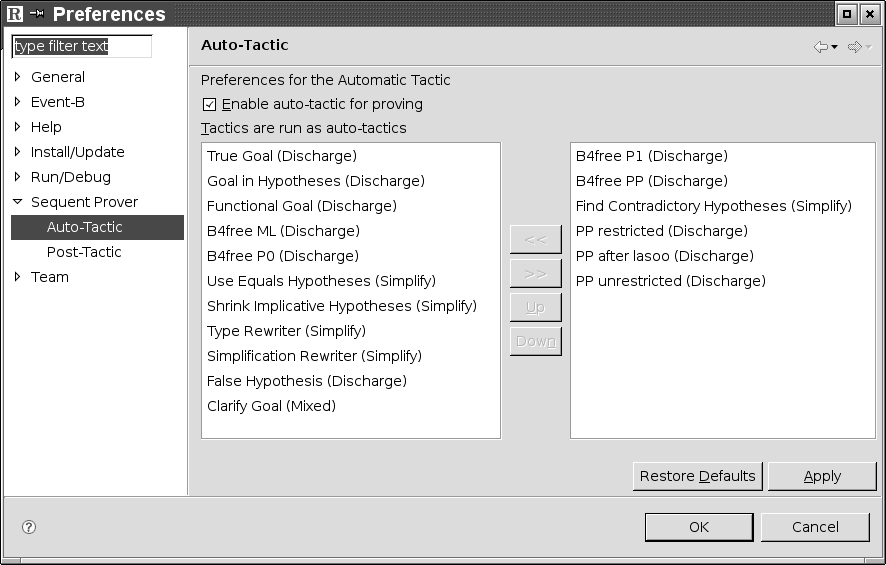
\includegraphics{img/reference/ref_10_auto_prover_pref.png}
	\caption{Auto Prover Preferences}
	\label{fig_ref_10_auto_prover_pref}
\end{center}
\end{figure}

On the left part you can see the ordered sequence of individual tactics composing the auto-prover, whereas the right part contains further tactics you can incorporate in the left part. By selecting a tactic you can move it from on part to the other or change the order in the left part.
Section~\ref{proof_tactics} gives an overview about what proof tactics are and 
  which are available.

\subsubsection{The Search Hypotheses View}
\index{view!Search Hypotheses}

By typing a string in the \textsf{Proof Control} view and pressing the \textsf{Search Hypotheses} (\icon{rodin/sh_prover.png}) button, a window is provided which contains all the  hypotheses that have a character string in common with the one entered by the user in the editing area. For example, if we search for hypotheses involving the character string ``cr", then after pressing the \textsf{Search Hypothesis} (\icon{rodin/sh_prover.png}) button on the \textsf{Proof Control} view, we obtain the windows as shown in Figure \ref{fig_ref_01_proving_perspective7}. 

\begin{figure}[!ht]
\begin{center}
	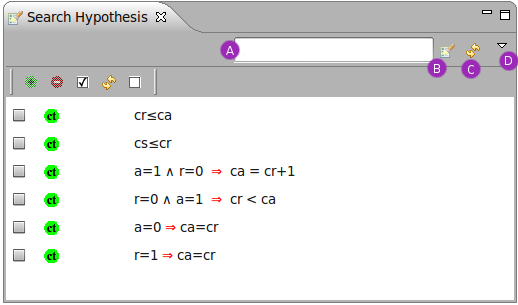
\includegraphics{img/reference/ref_01_proving_perspective7.png}
	\caption{The Search Hypotheses View}
	\label{fig_ref_01_proving_perspective7}
\end{center}
\end{figure}

This view also integrates a ``quick search" area (A), that allows us to search quickly hypotheses involving short character strings such as ``cr", a search hypothesis button (B) that behaves the same as the button of the proving window, a refresh button (C) that updates the window manually for more control, and a drop down menu (D) to set the preferences of the view up.

By pressing return key or the button (B) (once a short string has been entered into the input area (A)), hypotheses can be searched quickly as if we used the Proof Control as described before.

The drop down menu (D) allows some preferences about the searched hypotheses to be set.

If we change preferences for the search, we might need to manually ``update'' the view with the button (C). By selecting the ``Consider hidden hypotheses in search" option, we can review all hypotheses that have been unselected in the \textsf{Selected Hypotheses} window.

To move hypotheses to the \textsf{Selected Hypotheses} window, select the wanted hypothesis (using the check boxes) and press the \icon{rodin/add.png} button. Adding these hypotheses to the selected hypotheses means that they will be visible to the prover. They can then be used during the next interactive proof phase.

To remove hypotheses from the \textsf{Search Hypotheses} window, use the \icon{rodin/remove.png} button. This button also appears above the selected hypotheses and allows the user to remove any hypothesis from the \textsf{Selected Hypotheses} window.

The other button, situated to the left each hypotheses, is the \icon{rodin/falsify_prover.png} button. Clicking on this will attempt a proof by contradiction. The effect is the same as if the hypothesis were in the \textsf{Selected Hypotheses} window. 

\subsubsection{The Cache Hypotheses Window}

This window allows the user to keep track of recently manipulated (i.e., used, removed, or selected) hypotheses for any PO. For example, when the user applies a rewrite to a hypothesis, a new hypothesis (after the rewriting) is selected, and the original hypothesis is deselected and put in the \textsf{Cache Hypotheses} window.

Similar operations (to that of the \textsf{Selected Hypotheses} and \textsf{Search Hypotheses} windows) such as removing, selecting and proof by contradiction (ct) are also available for the cached hypotheses. Interactive proof steps (e.g., rewriting) can also be carried out from the \textsf{Cache Hypotheses} window.

\subsubsection{Proof Information View}

This view displays information so that the user can relate a proof obligation to the model. For example, typical information for an event invariant preservation includes the event as well as the invariant in question. For instance in Figure \ref{fig_ref_01_proving_perspective8}, the hyperlinks \textsf{CreateToken} and \textsf{inv2} can be used to navigate to the containing machine. 

\begin{figure}[!ht]
\begin{center}
	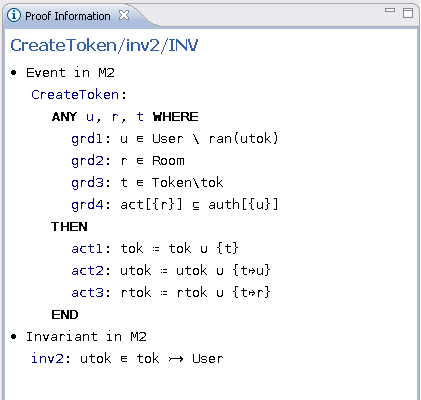
\includegraphics{img/reference/ref_01_proving_perspective8.png}
	\caption{Proof Information View}
	\label{fig_ref_01_proving_perspective8}
\end{center}
\end{figure}

\subsubsection{Rule Details View}

This view displays the information relating to a given proof tree node onto which a rule was applied.
A command is available when right-clicking on a proof tree node in order to reveal the \textsf{Rule Details} view (See Figure \ref{fig_ref_01_proving_perspective9}).

\begin{figure}[!ht]
\begin{center}
	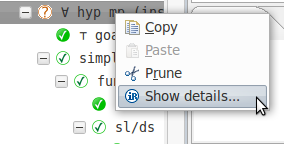
\includegraphics{img/reference/ref_01_proving_perspective9.png}
	\caption{Open Rule Details View}
	\label{fig_ref_01_proving_perspective9}
\end{center}
\end{figure}

By default, this view is a fast view. If the window does not appear, seek the button (identified by the view's icon) at the bottom left of the workbench to make this view visible.

Figure \ref{fig_ref_01_proving_perspective10} gives an overview of the \textsf{Rule Details View}.

\begin{figure}[!ht]
\begin{center}
	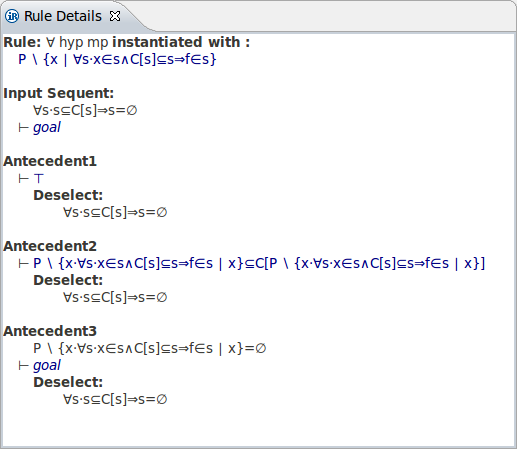
\includegraphics{img/reference/ref_01_proving_perspective10.png}
	\caption{Rule Details View}
	\label{fig_ref_01_proving_perspective10}
\end{center}
\end{figure}

A quick summary of the applied rule contents is provided. In this figure, we display the contents of the rule named \textsf{$\forall$ hyp mp}, where an input has been used to instantiate an hypothesis. One can quickly see the input that was used to instantiate the rule (the line below \textsf{Rule: $\forall$ hyp mp instantiated with:}), and the hypothesis that was considered by this rule (the line below \textsf{Input Sequent:}). Furthermore, it is possible to view the antecedents created by this rule in details (i.e. child proof tree nodes) and the actions performed on the hypotheses (selection, deselection, etc.). 

\subsubsection{Auto-tactic and Post-tactic}
\index{auto-tactic}
\index{post-tactic}
\index{tactics!auto-tactic}
\index{tactics!post-tactic}

The auto-tactic automatically applies a combination (i.e. ordered list) of rewrite tactics, inference tactics and external provers to newly generated proof obligations. However, they can also be invoked by the user by clicking on the \icon{rodin/auto_prover.png} button in the \textsf{Proof Control} view. Note that the automatic application of the auto-prover can be quickly toggled with the \textsf{Prove Automatically} menu item available from the \textsf{Project} menu (See Figure \ref{fig_ref_01_proving_perspective11}).

\begin{figure}[!ht]
\begin{center}
	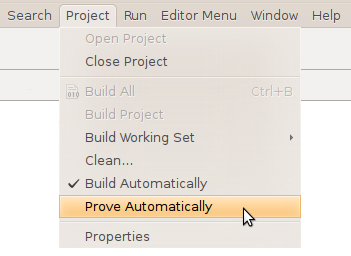
\includegraphics{img/reference/ref_01_proving_perspective11.png}
	\caption{Toggle auto-prover via project menu}
	\label{fig_ref_01_proving_perspective11}
\end{center}
\end{figure}

The post-tactic is also a combination of rewrite tactics, inference tactics and external provers and is applied automatically after each interactive proof step. However, it can also be invoked manually by clicking on the \icon{rodin/broom_prover.png} button in the \textsf{Proof Control} view.

Note that the post-tactic can be disabled quickly by clicking on the little arrow (marked with an A) of the \textsf{Proof Control} view (right upper corner) and then on \textsf{Disable post-tactic} option (B) as shown in figure \ref{fig_ref_01_proving_perspective12}.

\begin{figure}[!ht]
\begin{center}
	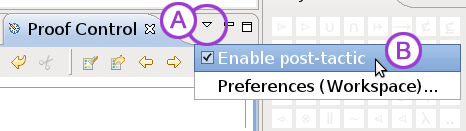
\includegraphics{img/reference/ref_01_proving_perspective12.png}
	\caption{Proof Control view menu}
	\label{fig_ref_01_proving_perspective12}
\end{center}
\end{figure}

\paragraph{Principles}

The ordered list of rewrite tactics, inference tactics and external provers that should be applied is called a profile. There are two default profiles. One is for auto-tactics and one is for post-tactics. These default profiles are immutable in time but can be duplicated for further modification by the user. The user can edit a profile and select it to run as automatic or post tactic. The idea is to have a set of available tactic profiles to be used as needed. Moreover, these edited profiles are shipped with projects if defined at the project level or can be imported or exported if defined at a workspace level. This makes it easy to share the profiles. 

There are two ways to run the automatic or post tactics:

\begin{itemize}
	\item Manually by clicking on the \icon{rodin/auto_prover.png} button or the \icon{rodin/broom_prover.png} button in the \textsf{Proof Control view} to launch the auto-tactic (with the selected auto-tactic profile) and the post-tactic (with the selected post-tactic profile) respectively.
	\item Automatically if such preference is activated. (Auto-tactic will then run after each proof step and post-tactic will run after each step and rebuild). Post-tactics and auto-tactics only need to be activated in order to run automatically (see previous sections on how to activate auto- and post-tactic). 
\end{itemize}

The user can separately define tactic profiles and assign them to post and auto tactics. Therefore, there are two tabs in the \textsf{Auto/Post Tactic} preference page for each of these choices. These tabs will be described in Section \ref{ref_01_preferences_auto_post_tactic}. 

\subsection{Preferences}
\label{preferences}
\index{preferences}

Rodin provides several options to set preferences the Event-B editor. You can access the preferences via \textsf{Window $\rangle$ Preferences $\rangle$ Event-B} in the menu bar. The following subsections describe the different preference option.

\subsubsection{Appearance}

This section provides settings for the Event-B editor appearance.

\paragraph{Colours and Fonts}

The colour and fonts preference page allows you to set the text and comment colour of the Event-B editor. Furthermore, it allows to toggle on or off the borders of the different fields in the Event-B editor. Figure \ref{fig_ref_01_preferences13} shows the Colours and Fonts preference page.

\begin{figure}[!ht]
\begin{center}
	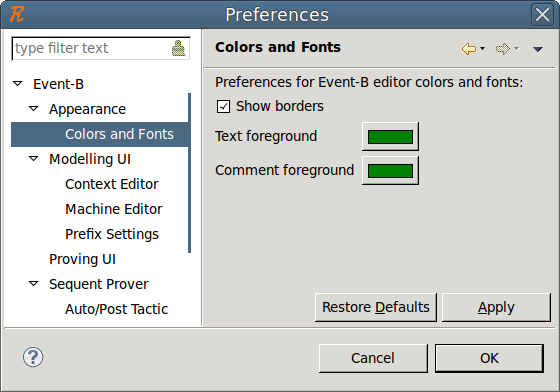
\includegraphics{img/reference/ref_01_preferences13.png}
	\caption{Colours and Fonts preferences}
	\label{fig_ref_01_preferences13}
\end{center}
\end{figure}

\subsubsection{Context and Machine Editor}

The context and machine editor preference pages allows you to customize the visible tabs of the context and machine editor.

\subsubsection{Prefix Settings}
\index{preferences!prefix}

This page describes the mechanism used to set element prefixes and perform renaming using dedicated actions for both machines and contexts. Note that prefixes are used for automatic renaming when elements should be alphanumerically ordered as well as when new elements are created. 

%\paragraph{Principles}

%This mechanism is close to eclipse preferences and properties settings. In our case, the prefixes are in any case, defined globally for a workspace scope. If the user does not set specific settings for prefixes at the workspace scope, the default prefixes which are given by elements contributions are used. Moreover, if the user changes the prefixes once, they will then be persisted. The new feature is here the ability for one to set up some specific settings for prefixes at a project scope. The settings will be then persisted through a file attached to the project settings (i.e., the prefixes used will be shared at export).

%\paragraph{Summary}

%\begin{itemize}
%	\item Default prefixes correspond to Rodin's default values,
%	\item A user can modify workspace settings via "Window" > "Preferences" menu,
%	\item Workspace modifications are persisted from one session to another,
%	\item Project specific settings can be set up and will then be persisted in a project scope,
%	\item Restoring default prefixes for a project will enable the current workspace prefix settings,
%	\item Restoring default prefixes for the workspace will reset the prefixes to their original values corresponding to the values which are set at Rodin's %%first launch.
%\end{itemize}

%\paragraph{Overview}

Figure \ref{fig_ref_01_preferences1} shows that modifying prefixes on the workspace level or on the project level will affect the names used at creation of new Event-B elements. One can see that the prefixes for variables and invariants, which were originally set to ``var" or ``inv'', have been replaced by ``variable" and ``invariant". New elements are then named using those prefixes.

\imagedpi{img/reference/ref_01_preferences1.pdf}{135mm}{img/reference/ref_01_preferences1.png}{Prefix Settings}{fig_ref_01_preferences1}

%\begin{figure}[!ht]
%\begin{center}
%	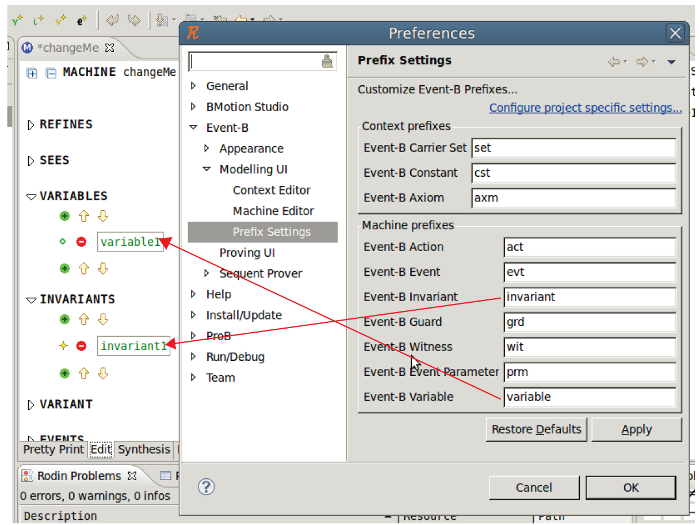
\includegraphics{img/reference/ref_01_preferences1.png}
%	\caption{Prefix Settings}
%	\label{fig_ref_01_preferences1}
%\end{center}
%\end{figure}

\paragraph{How to set prefixes}

Prefix settings can be accessed through in two different ways depending on the scope of their application: \textsf{Window $\rangle$ Preferences $\rangle$ Event-B $\rangle$ Modelling UI $\rangle$ Prefix settings} or directly via, \textsf{Rename $\rangle$ Customize prefixes...}.

\paragraph{Project specific settings}

The user can select profiles locally for a project. To do so, you can select the \textsf{Prefix Settings} property page available via right-click on a project and select the \textsf{Properties} item. You can also click on the \textsf{Configure project specific settings} link on the \textsf{Prefix Settings} preference page. In this case, one will have to choose the project for which the prefixes should be set up. This is allowed via a specific project selection dialog. After the project selection, a dialog for prefix settings opens for the selected project. 

A window (see Figure \ref{fig_ref_01_preferences2}) appears, where a page handling prefixes settings allows a user to customize prefixes for a chosen project. On this page, the user can toggle the button \textsf{Enable project specific settings}.

\begin{figure}[!ht]
\begin{center}
	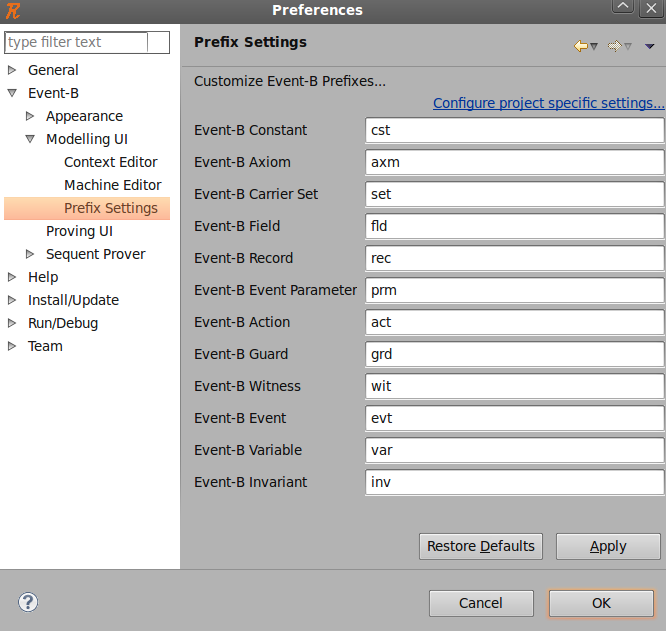
\includegraphics{img/reference/ref_01_preferences2.png}
	\caption{Project specific prefix settings}
	\label{fig_ref_01_preferences2}
\end{center}
\end{figure}

\begin{itemize}
	\item If this button is enabled, the prefixes used are those which are specified at this project level.
	\item If this button is not enabled, the prefixes used are those which are defined at the workspace level. 
\end{itemize}

\subsubsection{Sequent Prover / Auto/Post Tactic}
\label{ref_01_preferences_auto_post_tactic}
\index{auto-tactic!preferences}
\index{preferences!tactics}
\index{post-tactic!preferences}
\index{tactics!auto-tactic}
\index{tactics!post-tactic}

\paragraph{Preferences for the selected auto and post tactic profile}

This section describes the \textsf{Auto/Post Tactic} tab of the \textsf{Auto/Post Tactic} preference page.

There are two scopes to set up preferences for the auto and post tactics: the workspace level and the project level. Note that if the automatic application of tactics is decided only at the workspace level, this option will also be set for the project level.

To access these preferences, open the ``Auto/Post Tactic" preference page that can be found after \textsf{Window $\rangle$ Preference $\rangle$ Sequent Prover}.

Figure \ref{fig_ref_01_preferences7} shows the \textsf{Auto/Post Tactic} preference page.

\begin{figure}[!ht]
\begin{center}
	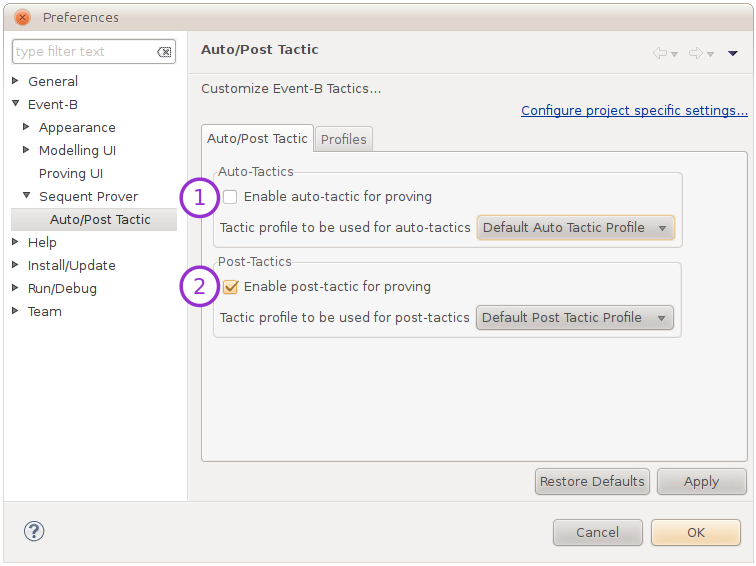
\includegraphics{img/reference/ref_01_preferences7.png}
	\caption{The ``Auto/Post Tactic" preference page}
	\label{fig_ref_01_preferences7}
\end{center}
\end{figure}

The buttons 1 and 2 are activating/deactivating the automatic use of auto- and post-tactics. Here you can also choose the profile that should be used for auto- and post-tactics. Note that there is always a profile selected, and this profile can be changed regardless of whether the tactics are automatically launched or not because there is always a way to manually launch auto- and post-tactics. On the previously references figure, the \textsf{Default Auto Tactic Profile} is used for the automatic tactic, and the \textsf{Default Post Tactic Profile} is used for the post-tactic.

%Figure \ref{fig_ref_01_preferences8} shows the "Auto/Post Tactic" reference page with both auto-tactic and post-tactic to automatically run, and where the user selects the profile "MyFirstTacticProfile" to be used as auto-tactic profile. 

%\begin{figure}[!ht]
%\begin{center}
%	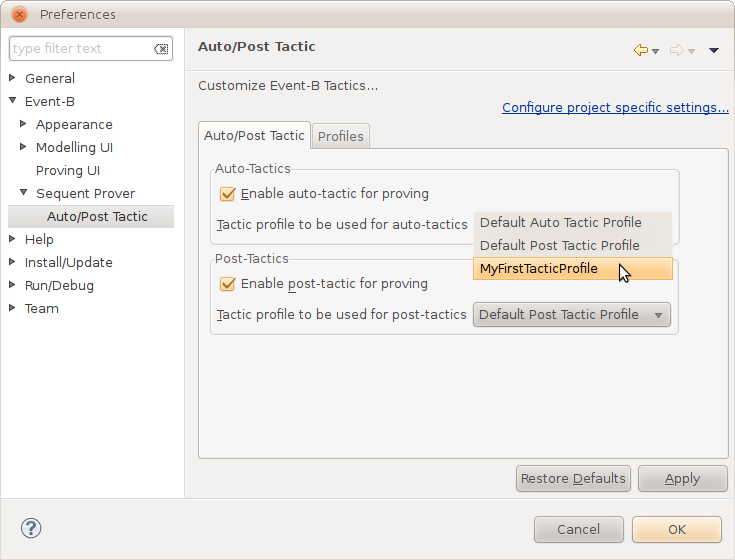
\includegraphics{img/reference/ref_01_preferences8.png}
%	\caption{Selecting a profile for the Auto-Tactics}
%	\label{fig_ref_01_preferences8}
%\end{center}
%\end{figure}

\paragraph{Preferences for available profiles}
\index{preferences!profile}

This section describes the \textsf{Profile} tab of the \textsf{Auto/Post Tactic} preference page. 

Figure \ref{fig_ref_01_preferences9} shows the contents of the profile tab. There are two visible lists: a list of profiles on the left and the tactics or provers that compose these profiles (Profile Details). Here one can see the contents of the default Auto Tactic Profile.

\begin{figure}[!ht]
\begin{center}
	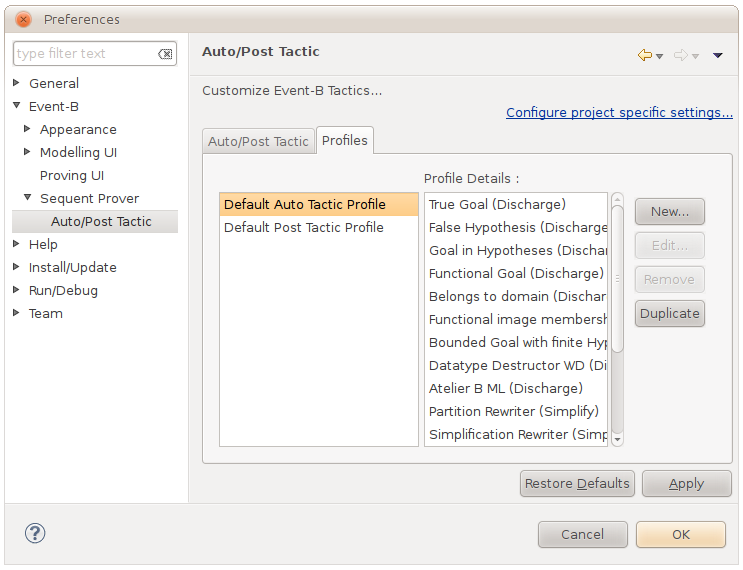
\includegraphics{img/reference/ref_01_preferences9.png}
	\caption{Selecting a profile for the Auto-Tactics}
	\label{fig_ref_01_preferences9}
\end{center}
\end{figure}

There are 4 buttons available to the user:

\begin{itemize}
	\item New: to create a new profile ``from scratch",
	\item Edit: to edit an existing (editable) profile,
	\item Remove: to remove a profile definitively,
	\item Duplicate: to duplicate a selected profile for further slight modification.
\end{itemize}

Default profiles can not be edited nor removed. That is why they this option appears in gray on the previously referenced figure.

Figure \ref{fig_ref_01_preferences10} shows the dialog available to edit or create a profile. For instance, here we create a profile named ``MyFirstTacticProfile".

\begin{figure}[!ht]
\begin{center}
	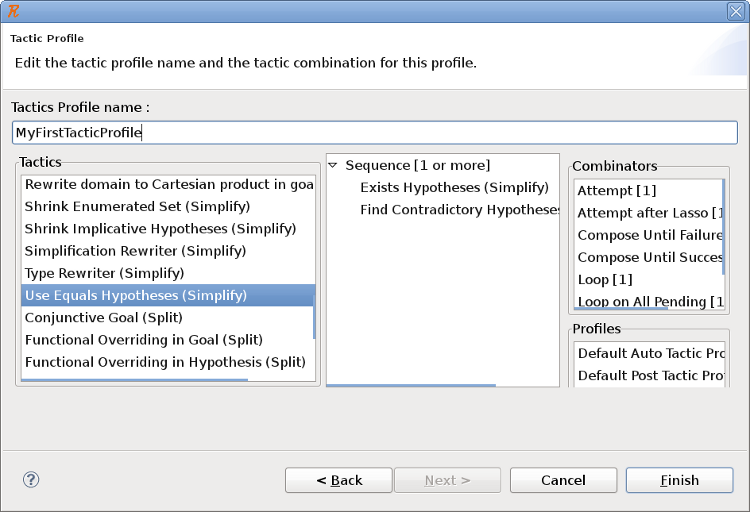
\includegraphics{img/reference/ref_01_preferences10.png}
	\caption{Selecting a profile for the Auto-Tactics}
	\label{fig_ref_01_preferences10}
\end{center}
\end{figure}

The list on the right represents the available and unselected tactics. The list of the left displays the profile contents and shows the selected tactics that will be applied from the top to the bottom. The user can choose a tactic from the list on the left and hit the \textsf{$>>$} button to select it or unselect some tactics from the list of the right using the \textsf{$<<$} button. The user can re-order the priority of the selected tactic using the \textsf{Up} and \textsf{Down} button. By clicking on \textsf{Finish}, the profile will be saved and available for use in the auto and post tactics.

\paragraph{Project specific settings}

The user can select profiles locally for each project. To do so, select the \textsf{Auto/Post Tactic} property page available via right-click on a project and select the  \textsf{Properties} item, or click the \textsf{Configure project specific settings link} on the \textsf{Auto/Post Tactic} preference page. Figure \ref{fig_ref_01_preferences11} shows what this \textsf{Auto/Post Tactic} tab looks like.

\begin{figure}[!ht]
\begin{center}
	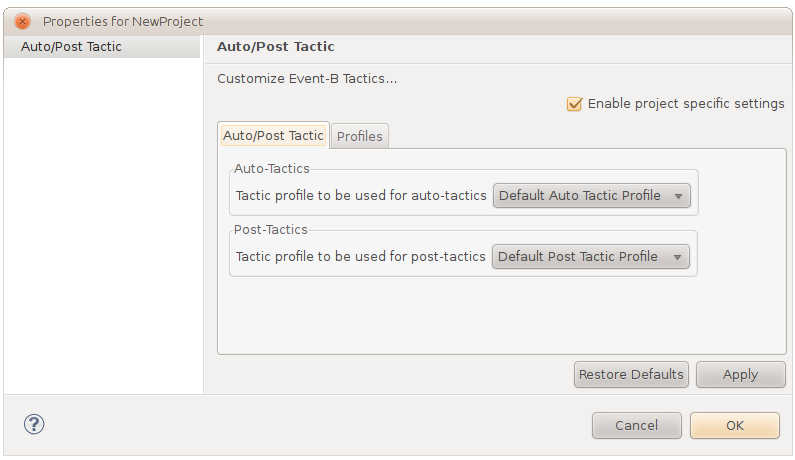
\includegraphics{img/reference/ref_01_preferences11.png}
	\caption{Auto/Post Tactic Tab for project specific settings for Auto/Post Tactic}
	\label{fig_ref_01_preferences11}
\end{center}
\end{figure}

Note that the enablement of automatic use of post and auto tactics is decided at the workspace level. Figure \ref{fig_ref_01_preferences12} shows the Profiles tab of the \textsf{Auto/Post Tactic} page for a project specific setting. At the project level, there is a contextual menu available via right click from the list of defined profiles. 

\begin{figure}[!ht]
\begin{center}
	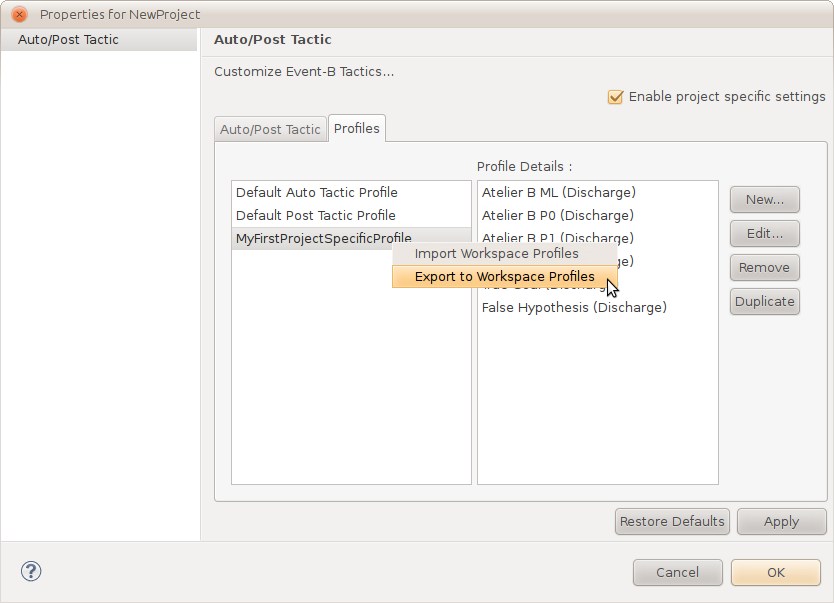
\includegraphics{img/reference/ref_01_preferences12.png}
	\caption{Profiles Tab for project specific settings for Auto/Post Tactic}
	\label{fig_ref_01_preferences12}
\end{center}
\end{figure}

This contextual menu offers two options to the user:

\begin{itemize}
	\item Import Workspace Profiles retrieve all the defined profiles in the workspace.
	\item Export to Workspace Profiles push a selected profile up in the list of workspace profiles.
\end{itemize}

\subsubsection{Preferences for the automatic tactics}
\label{preferences_for_the_automatic_tactics}
\index{auto-tactic}
\index{preferences!tactics}
\index{auto-tactic!preferences}

\paragraph{Introduction}

The purpose of this section is to give a more detailed preferences to the user so he can build his own automated tactics. More precisely, the user should have a way to specify which parameters have to be passed to the reasoners and have a way to construct complex proof strategies.

\paragraph{User Documentation}

Here is the documentation about the current implementation of the Auto-tactic and Post-tactic preferences.

\paragraph{Tactic Combinators}

Tactic combinators can be used to construct complex proof strategies.

Historically, one combinator has existed since the beginning of auto tactic preferences: the ``loop on all pending". It takes one or more tactics and loops them over every pending child until all tactic fail. Until Rodin 2.3 was released, it was the only combinator in Rodin. It is used on the configurable list of auto and post tactics. Rodin 2.3 is easier to configure because there are several other combinators and auto tactic editors.

The following is a list of combinators present by default.

One may notice the absence of child-specific combinator (i.e. combinators that apply tactic T1 on the first child, T2 on the second child, etc.) even though this kind of combinator exists in other provers. The reason is that we are concerned mainly  auto tactics and these are tactics that are attempted in a general context. Provers with child-specific combinators are used to make manual proof because they require proof-specific adaptation.

\subparagraph{Composers}

A composer combinator applies its given tactic(s) to the given node. The given node may be open or closed. It succeeds if at least 1 tactic application is successful. 

\begin{center}
    \begin{tabular}{ | l | l | l | l | p{5cm} |}
    \hline
	Name & Arity & Description & Stops when  \\ \hline
	Sequence & 1..n  & applies given tactics in given order & all tactics have been applied  \\ \hline
	Compose until Success & 1..n  & applies given tactics in given order & a tactic application succeeds \\ \hline
	Compose until failure  & 1..n  & applies given tactics in given order & a tactic application fails \\ \hline
	Loop & 1 & applies given tactic repeatedly & the child tactic application fails \\ \hline
    \end{tabular}
\end{center}

\subparagraph{Selectors}

A selector combinator applies its given tactic to the set of nodes it selects. Selected nodes are computed from the given node. The given node may be open or closed. It succeeds if the tactic application is successful for at least 1 selected node. 

\begin{center}
    \begin{tabular}{ | l | l | l | p{5cm} |}
    \hline
	Name & Arity & Selects \\ \hline
	On all pending  & 1 & all pending children of the given node (the given node itself if it is open) \\ \hline
    \end{tabular}
\end{center}

\subparagraph{Post Actions}

A post actions applies its given tactic to the given node. The given node must be open (otherwise it fails). Then it performs a specific treatment which is guarded by a trigger condition. 

\begin{center}
    \begin{tabular}{ | p{1,5cm} | p{1cm} | p{6cm} | p{5cm} |}
    \hline
	Name & Arity & Trigger Condition & Post Action \\ \hline
	Attempt & 1 & the given node still has pending children (subtree not closed) & prune proof tree at given node  \\ \hline
    \end{tabular}
\end{center}

\subparagraph{Loop on All pending}

$loopOnAllPending(T_1 \ldots T_n) \;\;\defi\;\; loop(onAllPending(composeUntilSuccess(T_1 \ldots T_n)))$

\paragraph{Other Ideas}

    timeout: a post action of arity 1 (with duration as input): limits the time allocated for the tactic that it is applied to (fails after time has gone out)

    limitDepth: a post action of arity 1 (with depth as input): limits the proof tree depth for the tactic that it is applied to (prevents tree from growing beyond a given depth)

%%% Local Variables: 
%%% mode: latex
%%% TeX-master: "rodin-doc"
%%% End: 
